\chapter{Evaluation}\label{ch5}

The ecoap prototype implementation is used to evaluate the proposed system architecture for scalable and reliable IoT services. Benchmarks are performed against the state of the art CoAP implementation for both unconstrained and less constrained environments. The evaluation scenarios, however, can vary depending on the many different communication models in IoT applications, including pure server, pure client and complex logic combining both of them \cite{kovatsch2015scalable}. 

For instance, a service could consist of resource directories which are servers that manage the devices and provide discovery. The devices would first register themselves there by issuing a request and periodically update their status \cite{core_directory}. Then other devices and services could contact the resource directory server for lookups. The devices can also be servers while a cloud service takes the role of client and observes resources hosted on many devices for monitoring and sensing. A combination of the two such as the OMA LightweighM2M \cite{lwm2m} specification acts as a resource directory and proxy at the same time, which means it not only receives registration and look-up requests from devices, but also issues requests to the resources of the devices. The devices in such case take both roles as well, since they expose their data as resources while using requests to register with the service.

To better evaluate the scalability and reliability of the proposed implementation, the pure server scenario is chosen. It eases the comparison with the current mainstream CoAP implementation, Californium, which proved its scalability in server role as well.


%One goal of Californium is to host services that communicate with other endpoints. In the IoT, we expect endpoints to exchange small messages. We consider each request and response a single unit of information. For the endpoints that communicate with a server, the relevant factors are the number of information that can be exchanged per time and the latency. Whether it is a CoAP or an HTTP message that carries the information from one endpoint to another is of no importance for the application. We measure the throughput of a server as the average number of requests that it is able to handle per second. This chapter presents the results of our experiments with Californium, Old Californium, and five state-of-the-art HTTP servers. Therefore this evaluation also serves as a comparison between CoAP and HTTP as protocols in the service backend. We particularly evaluate the scalability of the seven servers with respect to the number of available cores and with respect to the number of endpoints that concurrently communicate with the server. A node In the World Wide Web usually is either in the role of a server or a client. Therefore, HTTP servers truly are servers only and are optimized for that purpose. For the sake of comparison, we concentrate our evaluation of Californium and Old Californium only on their role as server even though both can appear as clients as well.

%We distinguish between two use-cases in which a server reaches its maximum performance. First, there might be a few clients that send many requests to the server. Such a client might be a proxy, for example, that in fact forwards requests from many clients but represents itself to the server as one highly demanding client. If server and clients used HTTP, they could keep a TCP connection alive and exchange many messages over it. In the second case, there are a large number of clients, each sending only a single request to the server. For an HTTP server, this means that each client establishes a new TCP connection only to exchange one request and immediately terminate it again. This is the scenario for a resource directory (RD). An RD can be thought of as an address book for resources. A endpoint can for instance register its resources of a specific type at the RD and another endpoint that looks for such a resource might later retrieve its URI form the RD. To simulate this scenario, HTTP clients do not keep their TCP connections alive but reestablish it for each request. The distinction between these two use-cases is much more prominent for HTTP than for CoAP as there is no such thing as establishing a connection in CoAP and it makes no difference whether requests come from the same or many different clients.

\section{Experiment Setup}

It is considered that in a typical IoT scenario, many endpoints would exchange small messages with certain services, while each request and response is treated as a single, compact unit of information. Therefore the number of information that can be exchanged per time and latency are the most important factors for the measurement of a server. This chapter presents the results of the experiments with ecoap and Californium, with focus on the evaluation of scalability with respect to the number of available cores and with respect to the number of concurrently active endpoints that communicate with the server.  

\subsection{Benchmark Tool}

There is few benchmark tool for CoAP. The one used by Californium is CoAPBench \cite{coapbench}, which is a Java based application similar to ApacheBench \cite{apachebench} and can be distributed over multiple machines. It is decided to develop an Erlang counterpart which follows its test logic. This is for two purpose. Firstly, with the concurrency model of Erlang, the benchmark tool can achieve higher level of load on one node thus avoid using multiple machines and simplify the test process. Second and the most important, the original CoAPBench does not provide a clear latency tracking functionality which is necessary in this evaluation, while integrating one with CoAPBench is not a trivial task. It is easier to reuse the components of ecoap to satisfy such a requirement. 

Similar with CoAPBench, the Erlang benchmark tool uses virtual clients for concurrency factor. A virtual client is a simplified CoAP client which can be easily implemented as one Erlang process. It is argued that since CoAP is a connection-less protocol, it does not make a lot difference whether messages come from one endpoint or many endpoints. However the many virtual clients model shows more similarity to real world use cases since it not only simulates all independent endpoints but also obeys the stop-and-wait nature of the protocol. High message rates in the IoT usually comes from millions of devices sending occasionally with intervals in minute or hour, instead of a small number sending at very high rate constantly \cite{kovatsch2015scalable}. More importantly, the fault-tolerance of ecoap is built based on the assumption that the server communicates with endpoints each having a different identification (e.g. address). Therefore the virtual clients model also helps verify the fault tolerance behaviour in the experiment.

\begin{figure}[!htbp]
\centering
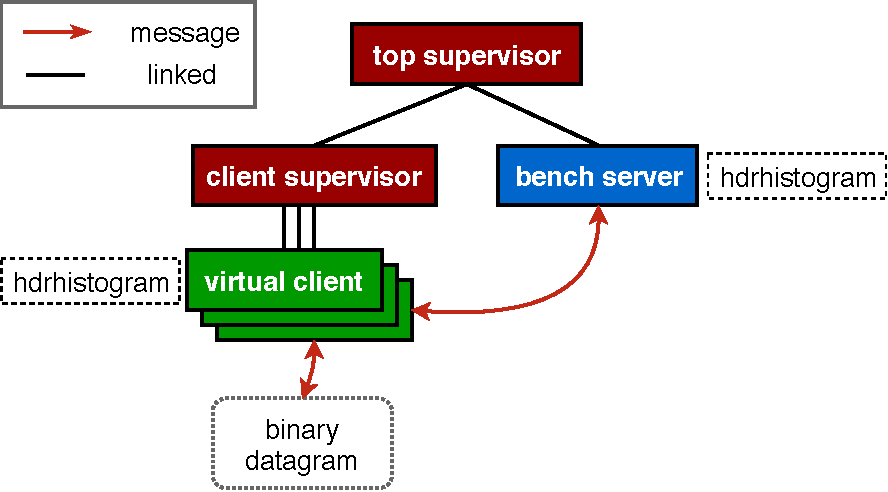
\includegraphics[scale = 0.55]{ecoap_bench_arch}
\caption[The supervision tree of the Erlang CoAP benchmark tool]{The supervision tree of the Erlang CoAP benchmark tool. A virtual client is a simplified CoAP client which only sends request in a closed-loop fashion, that is, waiting for a response before sending next request. Each virtual client holds a HDR histogram and records response time of every request it issued in it. The bench server process holds another HDR histogram which aggregates the contents of all virtual clients after a test has finished.}
\label{fig:ecoap_bench_arch}
\end{figure}

The benchmark tool works in a closed-loop fashion and adheres to basic congestion control. That is to say, each virtual client sends requests to the server as fast as it can handle them: it sends confirmable requests and always waits for the response before the next request is issued. Retransmission is disabled in order to not blur the number of sent and successfully handled requests. A timeout of 10 seconds is applied in case of a message loss, which is recorded in a separate counter. Round trip time fo each request is stored using the High Dynamic Range (HDR) Histogram \cite{hdr_erl}, which supports the recording and analyzing of sampled data value with dynamic range and pre-defined precision in constant memory footprint. An Erlang ports of the HDR Histogram is available. Thus statistically interesting measurements including minimum, maximum and percentile values can be accessed after each test. A brief architecture of the benchmark tool can be found in figure \ref{fig:ecoap_bench_arch}.

%While there are plenty of benchmark tools available for HTTP, to the best of our knowl- edge, there is none for CoAP. Therefore, we developed CoAPBench, a tool similar to ApacheBench31. It is part of our Californium framework, and hence publicly available to replicate our experiments.

%CoAPBench

%CoAPBench uses virtual clients to meet the defined concurrency factor. To have enough resources to saturate the server and keep all collected statistics in memory, CoAPBench can be distributed over multiple machines. A master controls the benchmark by establishing a TCP connection to all slave instances. We designed this master/slave mechanism to be able to execute third-party benchmark tools as well. Thus, we can run ApacheBench distributed and synchronized over multiple machines and bring even very powerful HTTP servers into saturation. Note that master and slaves only communicate before and after the experiment, so that the network traffic is not influenced by our tool.

%CoAPBench adheres to basic congestion control, that is, each CoAP client sends Confirmable requests and waits for the response before the next request is issued. We disable retransmissions, though, to not blur the numbers of sent and successfully handled requests. In case of message loss, a client times out after 10 seconds, records the loss in a separate counter, and continues with a new request.

\subsection{Setup}

All benchmarks are performed using the Erlang benchmark tool. The experiment environment varies depending on whether the server runs under constrained platform or not. It generally consists of one powerful client machine connected to the server through high speed network. Details of the machine specification are given for individual experiments respectively.

The main interest of this work is the server performance and scalability on handling the protocol instead of complex business logic. Therefore the server under test simply holds a \verb|/benchmark| resource which responds with a ``hello world" payload to GET requests. One can specify the number of concurrent virtual clients to be started during one test. All clients stress the server for 60 seconds with requests and then comes a 30 seconds cool-down interval. A growing number of concurrent clients are used here to achieve desired concurrency factor, which stepwise increases from 10 to 10,000. Test for each concurrency value is performed five times and the average value is recored.  

\section{Multi-core Scalability} \label{multi_core_scalability}

To evaluate whether the proposed prototype meets the design goal of scalability, the following experiment tests if ecoap scales well with an increasing number of CPU cores and concurrency factor. In detail, it measures the throughput under a cloud environment with different processor affinity settings, which are provided as Erlang runtime parameters. One can use the settings to specify the number of online schedulers of the Erlang virtual machine and whether they are bound to certain CPU cores.

The unconstrained cloud is chosen as target platform because it should better reveal the scalability of the system compared with a constrained one. Virtual machines hosted on Amazon Web Service (AWS) are used for the test since it is easier to be customized. In order to reduce the disturbance in such a virtual environment, all benchmarks run on dedicated instances \cite{aws_dedicated_instance} where no other users could share the resource simultaneously. The benchmark tool is running on a m4.4xlarge instance with 16 virtual CPUs and 64 GB of RAM, while the server is running on a m4.2xlarge instance with 8 virtual CPUs and 32 GB of RAM, both with Ubuntu Server 16.04 LTS installed. The two instances are connected to one subnet exclusively through enhanced networking (up to 25Gbps \cite{aws_instance}), as shown in figure \ref{fig:experiment_setting_aws}. 

\begin{figure}[!htbp]
\centering
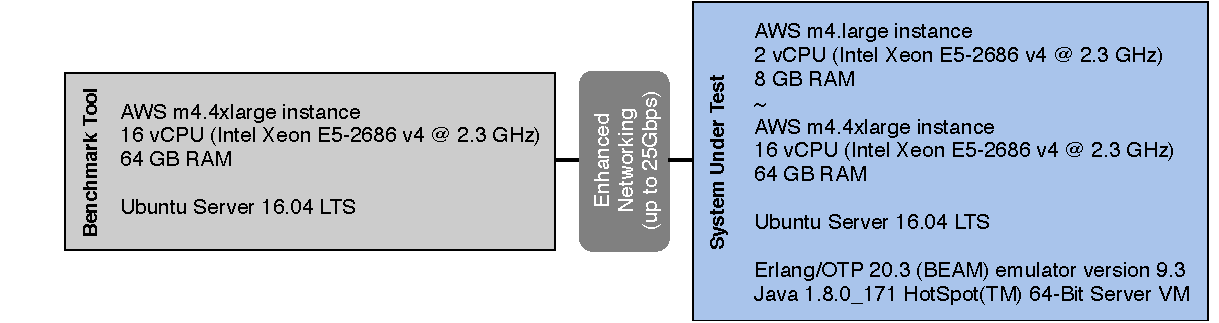
\includegraphics[scale = 0.55]{experiment_setting_aws}
\caption{Unconstrained experiment environment}
\label{fig:experiment_setting_aws}
\end{figure}

Since the server has to cache requests and corresponding responses to detect duplicates, the memory consumption soon becomes the the majority of the load. Though CoAP allows to relax duplicate detection for idempotent requests, it is decided to strongly reduce the lifetime of confirmable messages rather than completely disable the deduplication, because the latter removes most state management pressure which makes the experiment even further from any real world use case. As a result, the EXCHANGE LIFETIME is tweaked to 1.5 seconds which leaves the server enough time to clean up all history states during a test interval, meanwhile ensuring the state management still be a part of the ordinary server activity.

\begin{figure}[!htbp]
\centering
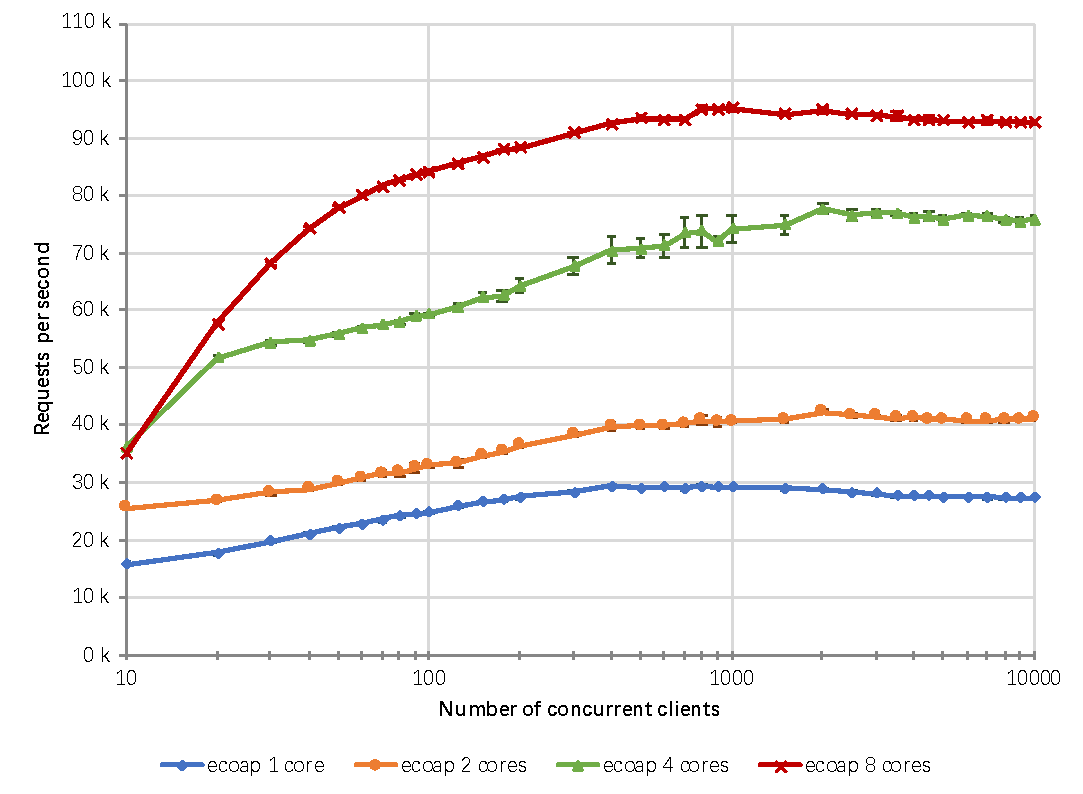
\includegraphics[scale = 0.8]{vertical_scalability}
\caption[Throughput for different numbers of assigned CPU cores on a 8 core m4.2xlarge AWS instance]{Throughput for different numbers of assigned CPU cores on a 8 core m4.2xlarge AWS instance. The server stay stable over an increasing concurrency factor with low latency.}
\label{fig:scalability}
\end{figure}

Figure \ref{fig:scalability} shows that the ecoap prototype scales well with the increasing number of available cores. The throughput curve reaches maximum of 95,172 requests per second when all 8 cores are available with a concurrency level of 1000 and stabilizes after it. ecoap almost doubles the performance when migrating from 1 cores to 2 cores and 2 cores to 4 cores. On 8 cores, it only performs about 1.3 times better than 4 cores. This is considered reasonable since not all tasks can be parallelized and the server prototype still suffers from single socket manager bottleneck. The latency follows similar pattern. Under the highest concurrency level (10,000 clients), the 95 percentile latency decreases from 91 milliseconds on 1 core to 37 milliseconds on 4 core, which is nearly 3 times lower.

\section{Throughput Verification}

In this section, the ecoap server prototype is evaluated against the state-of-the-art CoAP solution, Californium. Due to various limitations, the evaluation does not include other implementations. However, as a mainstream solution, Californium is proved to scale better than the majority implementations that are publicly available \cite{lanter2013scalability} \cite{kovatsch2014californium} \cite{kovatsch2015scalable}. Therefore, comparing the proposed implementation with Californium should be enough to assess its performance. 

\subsection{Unconstrained Environment}

First comes the evaluation in unconstrained environment. The experiment is taken in the same environment as the the previous one, that is, a m4.4xlarge instance with 16 virtual CPUs and 64 GB RAM as client and a m4.2xlarge instance with 8 virtual CPUs and 32 GB RAM as server. Same benchmark resource is hosted on both servers and the message lifetime is also tweaked for Californium. Maximum number of open file descriptors is increased to allow enough open UDP sockets. The socket buffer is increased to 1MB for both servers to reduce unnecessary message loss. The Erlang runtime is ordered to bind all schedulers to available CPU cores and use kernel poll provided by the operating system. 

\begin{figure}[!htbp]
\centering
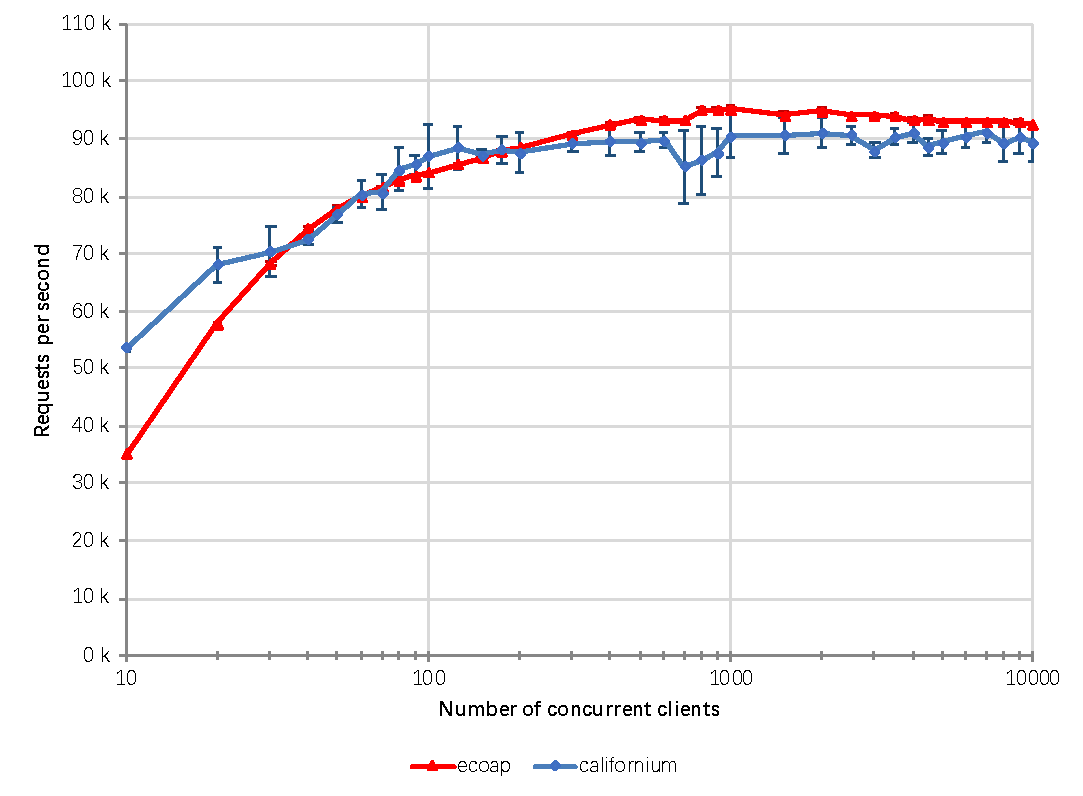
\includegraphics[scale = 0.8]{throughput}
\caption[Throughput comparison on a 8 core m4.2xlarge AWS instance]{Throughput comparison on a 8 core m4.2xlarge AWS instance. ecoap has same level of performance as Californium with slightly better peak throughput. Throughput of ecoap grows slower due to possible scheduling overhead introduced by the Erlang runtime. Californium suffers from a higher standard deviation, though.}
\label{fig:throughput}
\end{figure}

As seen in figure \ref{fig:throughput}, ecoap and Californium have close performance in terms of requests handled per second. Californium performs better at beginning than ecoap, which can be explained as the Erlang runtime brings more overhead for scheduling when there are not enough incoming requests to fully utilize all the schedulers. It increases the time processing a single request. Since the benchmark tool takes the same method as CoAPBench, the clients would wait for a request to finish before issuing the next one, making them spending more time waiting for the response. ecoap catches up at concurrency level of 40 and the throughput of both servers keep growing with the increasing number of concurrent clients. Californium stabilizes with around 150 clients while ecoap reaches its maximum capability after reaching 500 clients. ecoap has slightly better peak throughput at 95,172 requests per second versus 91,169 requests per second for Californium. Again, ecoap grows more slowly and requires more clients to saturate the server.

On the other hand, Californium has a high standard deviation during the test, as indicated by the error bars in the figure. The standard deviation is shown for ecoap as well, but is almost negligible. The performance curve of Californium is in general not as smooth as ecoap.
This may have many reasons. After observing the system resource consumption during the experiments, it is found that the Erlang runtime occupies more CPU and saturate faster than the Java Virtual Machine (JVM), while the JVM frees memory much slower than the Erlang one. As a result, Californium consumes much more memory than ecoap especially after long time testing. It is confirmed through both the Linux process viewer \verb|htop| and the \verb|jvisualvm| \cite{jvisualvm} virtual machine profiling tool. There is no related memory leak being observed though, as local test proved that message exchange states are successfully removed after corresponding lifetime. It is inferred that the JVM needs more time to invoke a full garbage collection with a large RAM, meanwhile the high concurrency level leads to large amount of objects being created and deleted frequently, which eventually influenced the performance of the server. In addition, the virtual environment on AWS might have undesired impact on the experiment. In contrast, the Erlang VM uses a per process generational garbage collection mechanism which runs inside each Erlang process independently, making the VM release resource sooner after finishing task and avoid stop-the-world freeze on applications as much as possible. 

\begin{figure}[!htbp]
\centering
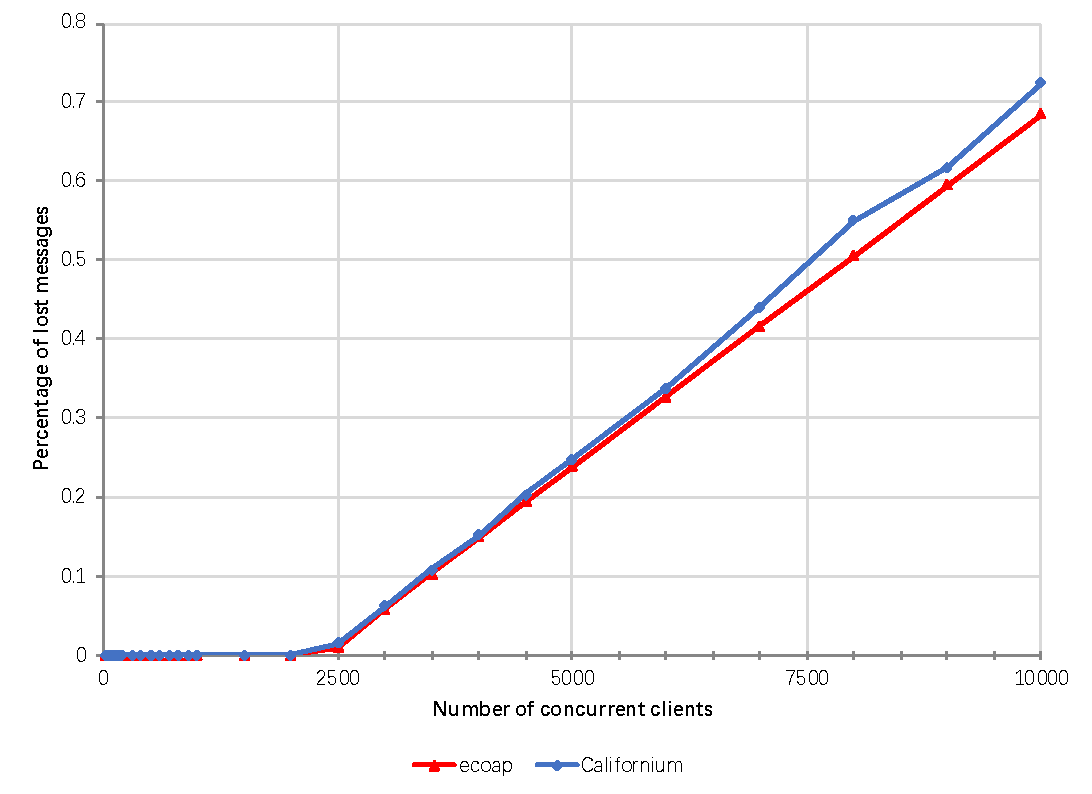
\includegraphics[scale = 0.8]{message_loss_rate}
\caption{Message timeouts by ecoap and Californium on a 8 core m4.2xlarge AWS instance}
\label{fig:message_loss_rate}
\end{figure}

Figure \ref{fig:message_loss_rate} gives the message loss through timeouts waiting for responses. With 2500 concurrent clients stressing the server, timeouts start to occur. The timeout rates rises with the increase of the concurrency factor to a maximum of about 0.7\% at 10,000 concurrent clients. Compared with the total amount of requests successfully served, the message loss rate is low enough and has negligible influence on the experiment . 

As mentioned before, Erlang uses various strategies to achieve soft-realtime, including the per process garbage collection. This has the most obvious impact on the latency of a high concurrency server. Figure \ref{fig:ecoap_min_round_trip_time} and figure \ref{fig:californium_min_round_trip_time} present the minimum round-trip time with respect to increasing concurrency factor, respectively. Though ecoap has more scattered results, both implementation get the response time around 2 milliseconds at maximum. However, as figure \ref{fig:ecoap_max_round_trip_time} and figure \ref{fig:californium_max_round_trip_time} show, the maximum round-trip time starts to vary.
The maximum round-trip time for ecoap is more concentrated and generally grows with the number of concurrent clients. The top value is around 300 milliseconds at concurrency level of 5000, which should be an acceptable delay for many time demanding applications. The maximum latency for Californium does not have an obvious rule and is usually an order of magnitude larger than ecoap. Some of them would cause a retransmission if it occurs in a real world use case. The phenomenon might be related to the high standard deviation discussed before, that is, due to garbage collection and memory management. 

But Californium does not always gives high latency. Figure \ref{fig:ecoap_95p_round_trip_time} and figure \ref{fig:californium_95p_round_trip_time} show the 95 percentile latency for both servers. The 95 percentile latency gives the value that is larger than 95\% of the entire dataset and is therefore a better metrics than pure average. As seen in the figures, both dataset increases almost linearly as the concurrency level goes up (since the x-axis is of logarithmic scale). Californium has a smaller maximum value of around 30 milliseconds after 2500 concurrent clients versus 35 milliseconds for ecoap also after 2500 clients. The latency values saturate at the same place because the network limit has been reached, since the timeouts also start to appear after this point. It seems that Californium could respond more requests only with a short delay than ecoap if one only considers the 95 percentile latency. However, the fair scheduling of Erlang ensures ecoap performs better in general especially with worst cases.

\begin{figure}[!htbp]
\centering
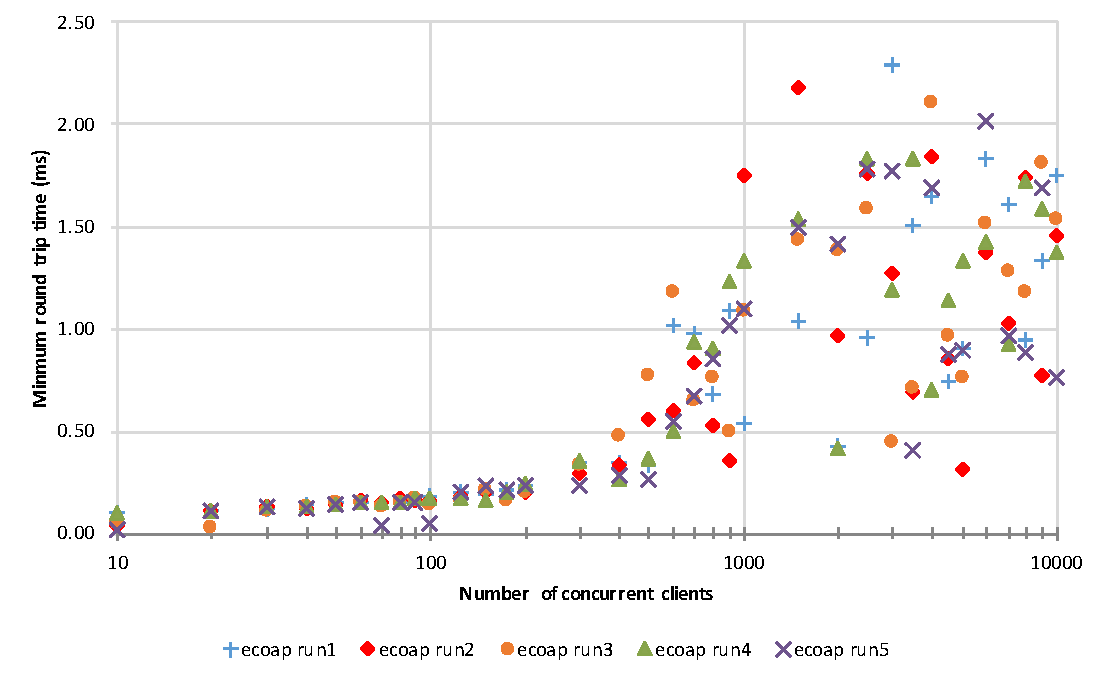
\includegraphics[scale = 0.8]{ecoap_min_round_trip_time}
\caption{Minimum round trip time of ecoap running on a 8 core m4.2xlarge AWS instance}
\label{fig:ecoap_min_round_trip_time}
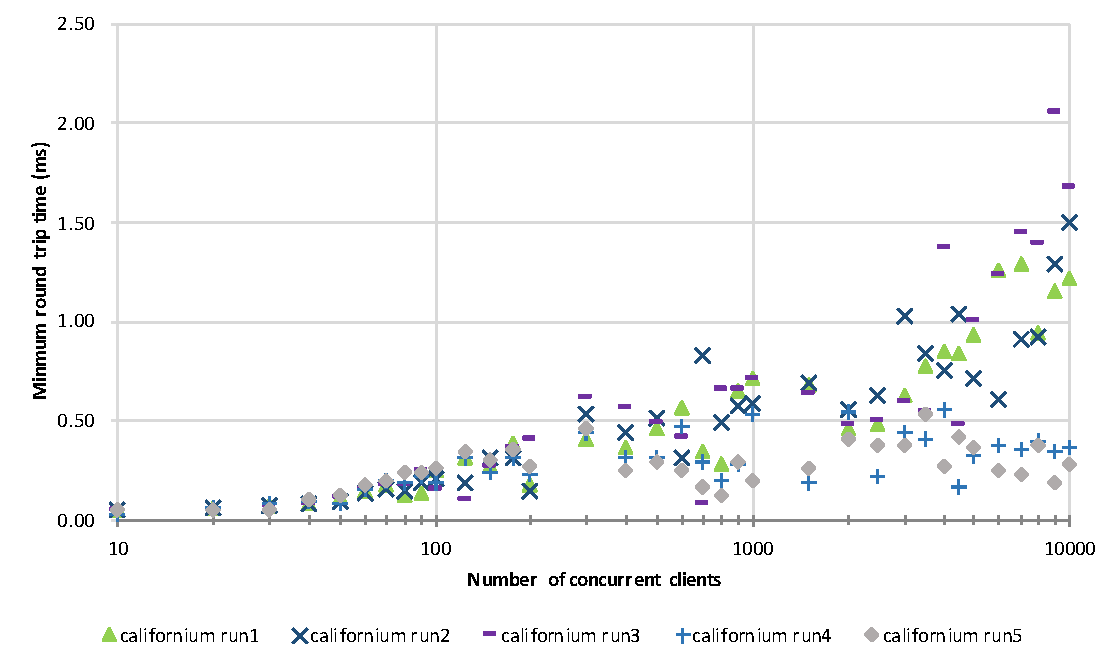
\includegraphics[scale = 0.8]{californium_min_round_trip_time}
\caption{Minimum round trip time of Californium running on a 8 core m4.2xlarge AWS instance}
\label{fig:californium_min_round_trip_time}
\end{figure}

\begin{figure}[!htbp]
\centering
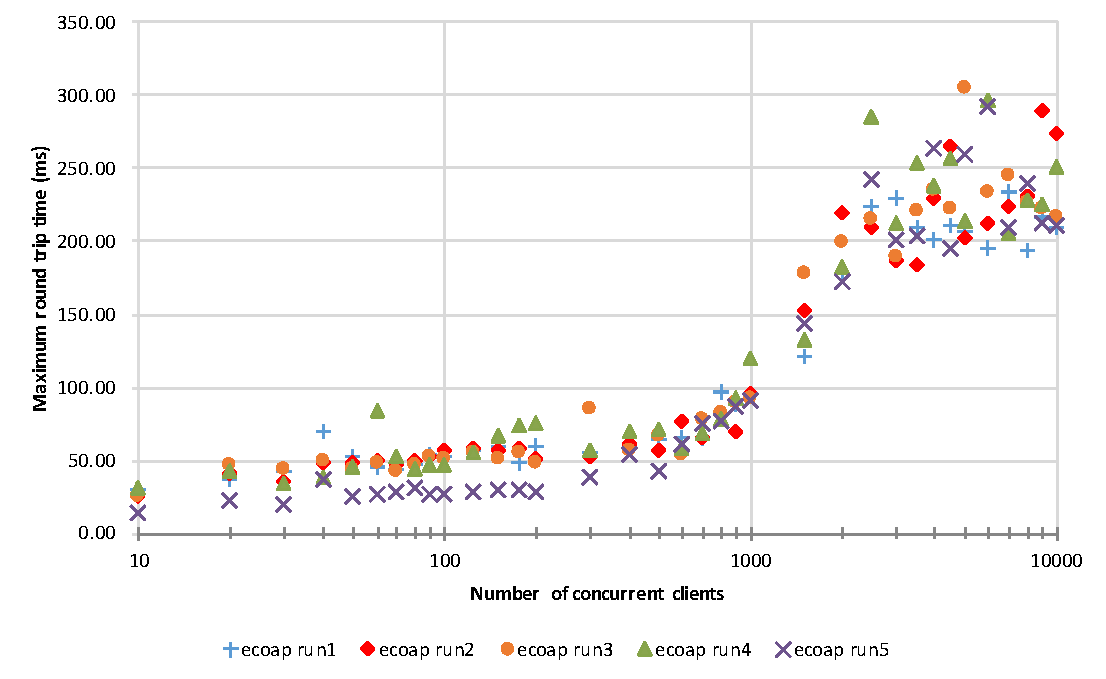
\includegraphics[scale = 0.8]{ecoap_max_round_trip_time}
\caption{Maximum round trip time of ecoap running on a 8 core m4.2xlarge AWS instance}
\label{fig:ecoap_max_round_trip_time}
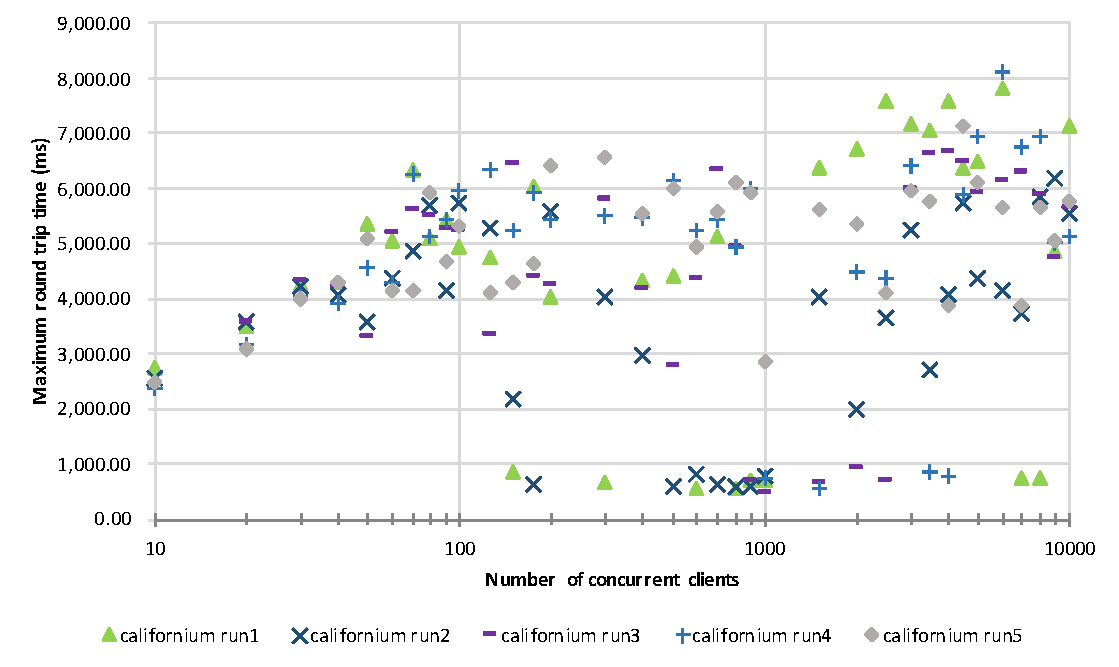
\includegraphics[scale = 0.8]{californium_max_round_trip_time}
\caption{Maximum round trip time of Californium running on a 8 core m4.2xlarge AWS instance}
\label{fig:californium_max_round_trip_time}
\end{figure}

\begin{figure}[!htbp]
\centering
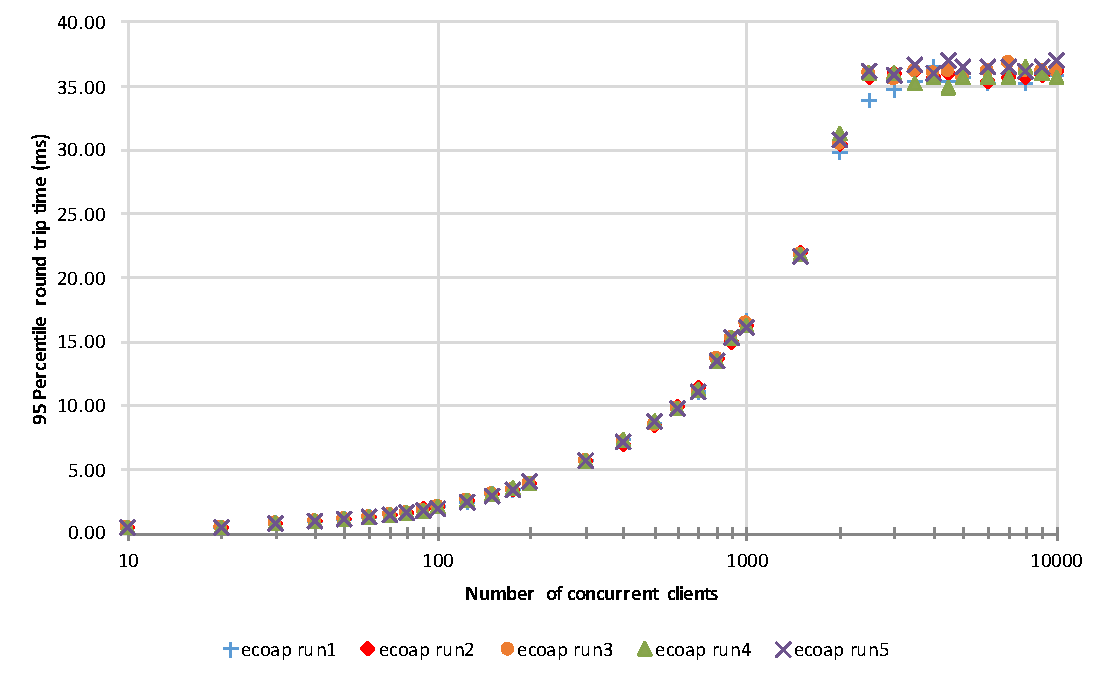
\includegraphics[scale = 0.8]{ecoap_95p_round_trip_time}
\caption{95 percentile round trip time of ecoap running on a 8 core m4.2xlarge AWS instance}
\label{fig:ecoap_95p_round_trip_time}
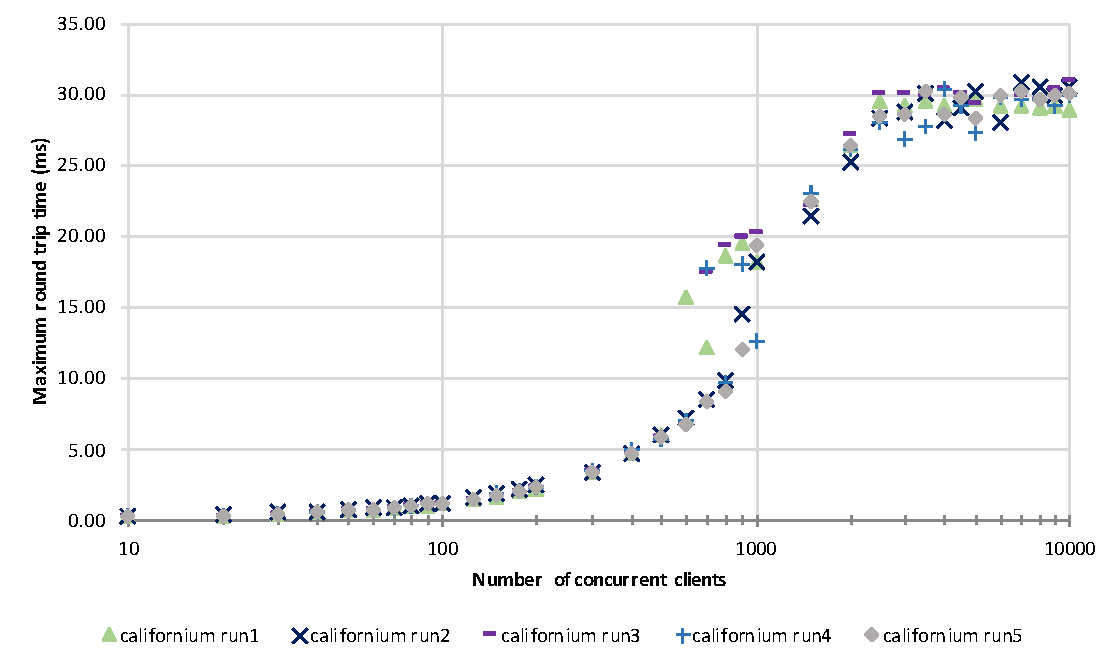
\includegraphics[scale = 0.8]{californium_95p_round_trip_time}
\caption{95 percentile round trip time of Californium running on a 8 core m4.2xlarge AWS instance}
\label{fig:californium_95p_round_trip_time}
\end{figure}

It can be seen that the proposed server prototype has comparable performance in terms of throughput and latency to the mainstream implementation, Californium, when being deployed  under cloud environment. The ecoap server scales well with increasing CPU cores and shows an advantage when general low latency is desired.

\subsection{Constrained Environment}

It is interesting to see to what extend a solution could scale up and scale down when being targeted to platforms with great capability difference. Hence, the same experiment is conducted under a more constrained environment, the Raspberry Pi 3 \cite{raspberry_pi}. The Raspberry Pi is essentially an embedded computer which can run Linux compatible applications. It is never as constrained as sensors and low-power devices, however, such type of platforms are still widely used as gateways or local processing unit in many IoT applications. For instance, it is ideal for running a Fog node that encapsulates more dummy sensors and devices.

The Raspberry Pi 3 is equipped with a quad-core 1.2GHz Broadcom BCM2837 64bit CPU, with 1GB RAM and BCM43438 wireless LAN and Bluetooth Low Energy (BLE) on board. The experiment environment consists of one Pi running the CoAP server and a MacBook Pro running the benchmark tool, connected via a Gigabyte network switch, as shown in figure \ref{fig:experiment_setting_rasp}. It is considered the MacBook Pro is powerful enough to generate loads that can saturate the Pi. 

\begin{figure}[!htbp]
\centering
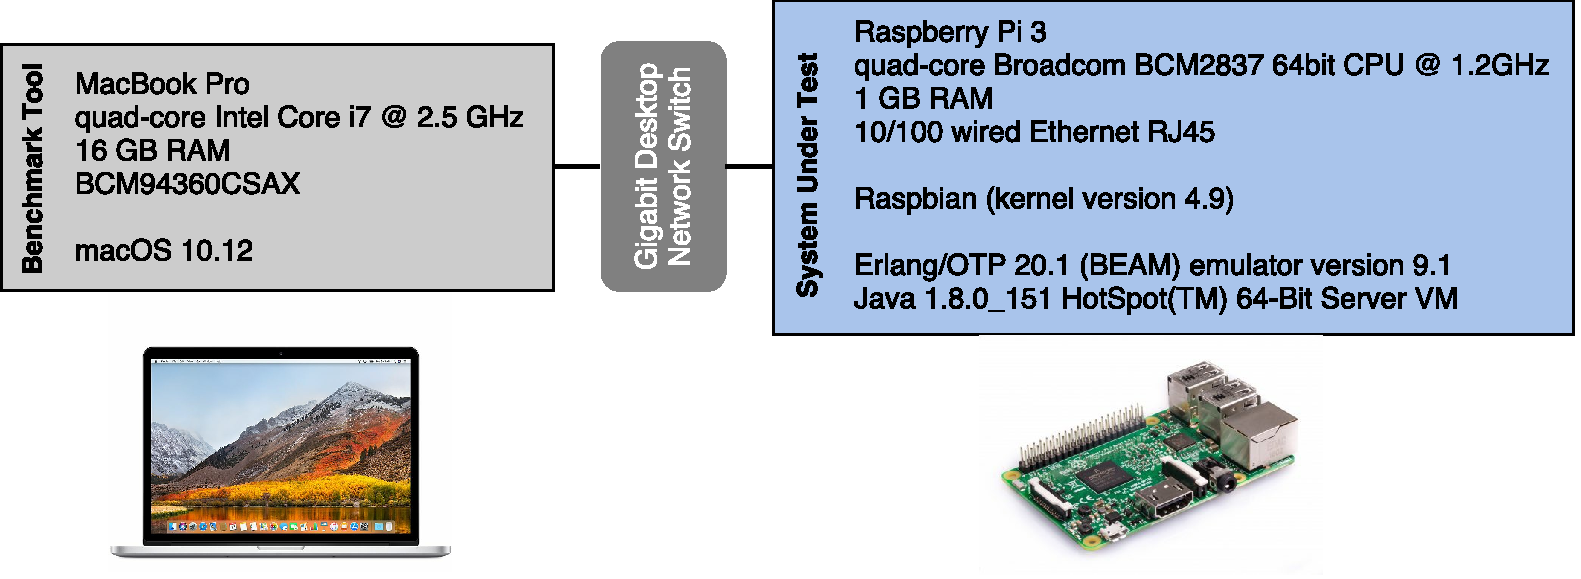
\includegraphics[scale = 0.55]{experiment_setting_rasp}
\caption{Constrained experiment environment}
\label{fig:experiment_setting_rasp}
\end{figure}

The test runs each server and measures its average throughput as well as latency, starting with 1 client and stepwise increasing the concurrency level to 10,000. It is of little interest to explore the vertical scalability on such a constrained platform. Therefore the server runs with all CPU cores enabled. All other settings including the server tweaking and socket buffer tuning are the same as the AWS experiment.

\begin{figure}[!htbp]
\centering
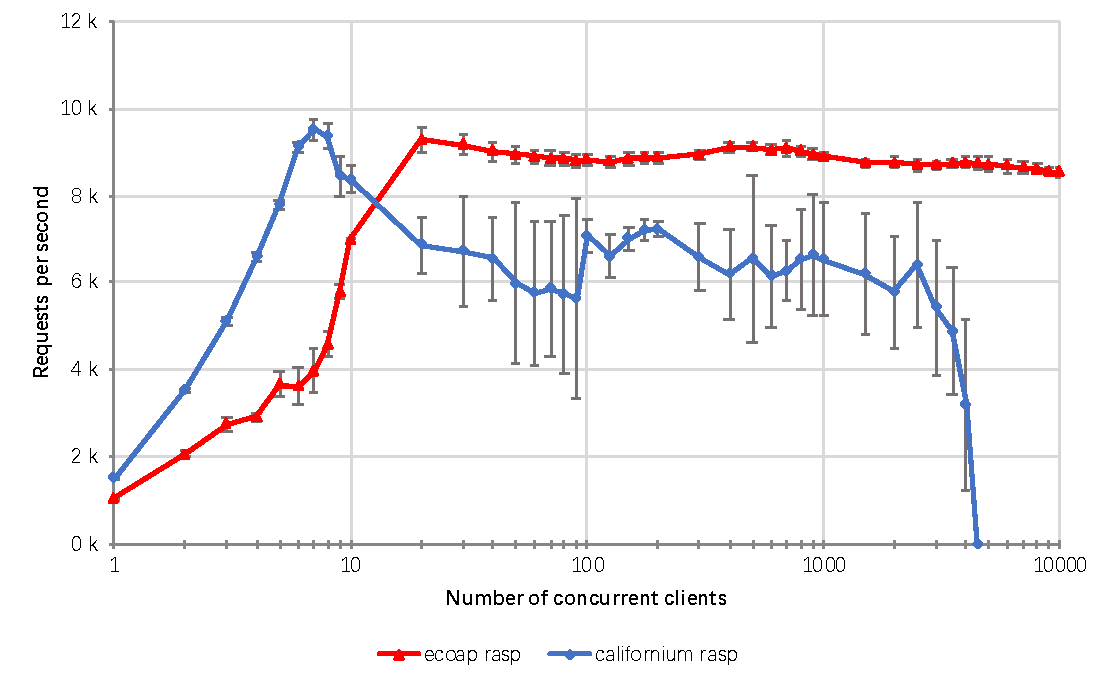
\includegraphics[scale = 0.8]{throughput_rasp}
\caption{Throughput comparison on a quad-core Raspberry Pi 3 at 1.2 GHz and 1GB RAM}
\label{fig:throughput_rasp}
\end{figure}

Figure \ref{fig:throughput_rasp} shows the throughput of the two servers on the Raspberry Pi. The performance curves are not as stable as the one under cloud environment. This might be due to the limit of the processing power of the Pi. ecoap achieves highest throughput with about 9000 requests per second. Interestingly, throughput of Californium grows quickly at low concurrency level but soon drops afterwards. The standard deviation is much higher than before, which implies it does not fully stabilize during the test. Californium eventually exits with an out of memory exception at the concurrency level of 4500. Without further investigation, it is not obvious why Californium crashes during the test. It is clearly not designed for constrained environment, but as stated in its introduction, Californium should also be able to run on embedded platforms such as an Android tablet, which has similar processing ability as the Raspberry Pi. Again, it is most likely that the underlying JVM can not manage memory efficiently within such a limited RAM under high concurrency load without further tuning and optimization. Several proofs can be found here. It is observed during the test that the JVM on Raspberry Pi starts in client mode by default, which renders the server crash at even lower concurrency level. Setting the VM to server mode and increase the heap size helps the server to run longer, but the 4500 clients is the final limitation here. 

The general result resembles the trend of the previous experiment. Figure \ref{fig:ecoap_min_round_trip_time_rasp} and figure \ref{fig:californium_min_round_trip_time_rasp} show the minimum latency clients can achieve in the experiment. When concurrency level is high, both servers need around 20-30 milliseconds at least to process a request, which is reasonably much slower than the cloud.
On the other hand, figure \ref{fig:ecoap_max_round_trip_time_rasp} indicates similar trend as the maximum latency of ecoap derived form the cloud experiment, though the largest value already exceeds 600 milliseconds. However, it is still more responsive compared with Californium, whose maximum latency is commonly over 2 seconds, as seen in figure \ref{fig:californium_max_round_trip_time_rasp}. When it comes to 95 percentile latency in figure \ref{fig:ecoap_95p_round_trip_time_rasp} and \ref{fig:californium_95p_round_trip_time_rasp}, performance of Californium is still acceptable, sometimes better than ecoap, until it hits a high concurrency factor. The ecoap server keeps stable during the intense stressing test with on average 3000 requests per second more than Californium and most requests are responded within 1 second even handling 10,000 concurrent clients.

\begin{figure}[!htbp]
\centering
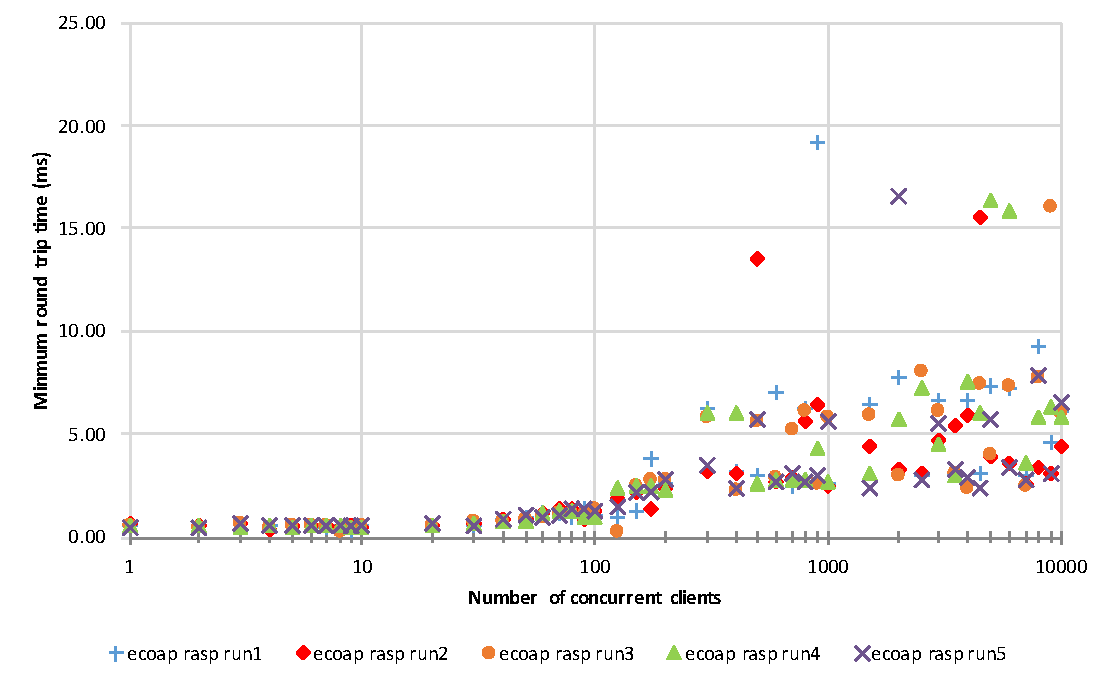
\includegraphics[scale = 0.8]{ecoap_min_round_trip_time_rasp}
\caption{Minimum round trip time of ecoap running on Raspberry Pi 3}
\label{fig:ecoap_min_round_trip_time_rasp}
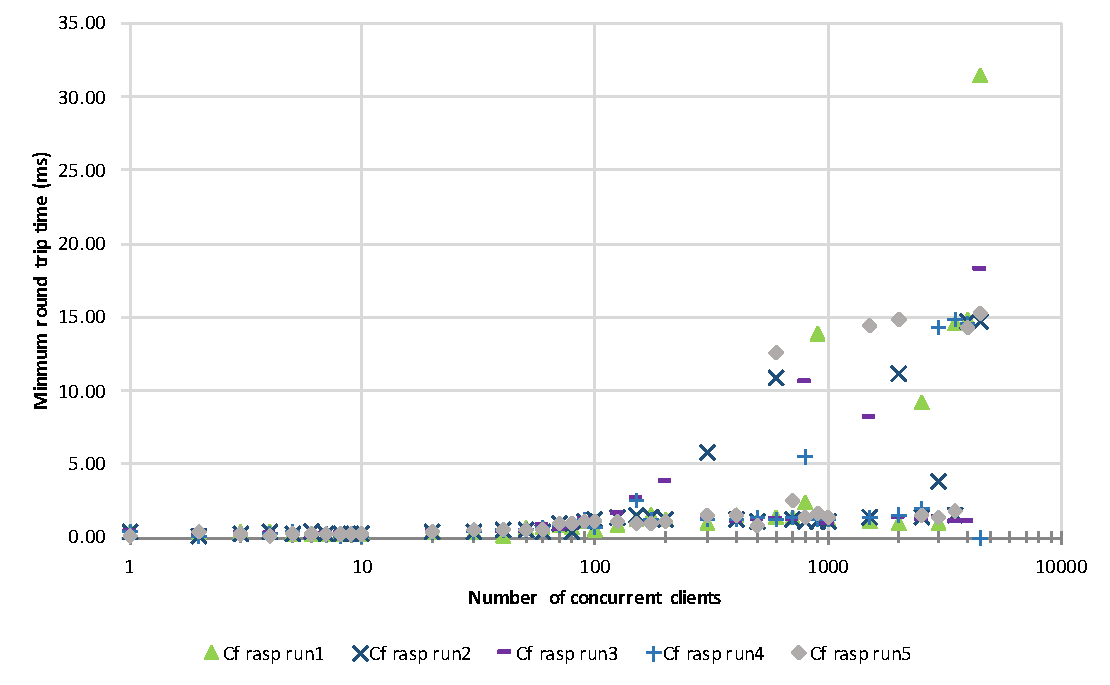
\includegraphics[scale = 0.8]{californium_min_round_trip_time_rasp}
\caption{Minimum round trip time of Californium running on Raspberry Pi 3}
\label{fig:californium_min_round_trip_time_rasp}
\end{figure}

\begin{figure}[!htbp]
\centering
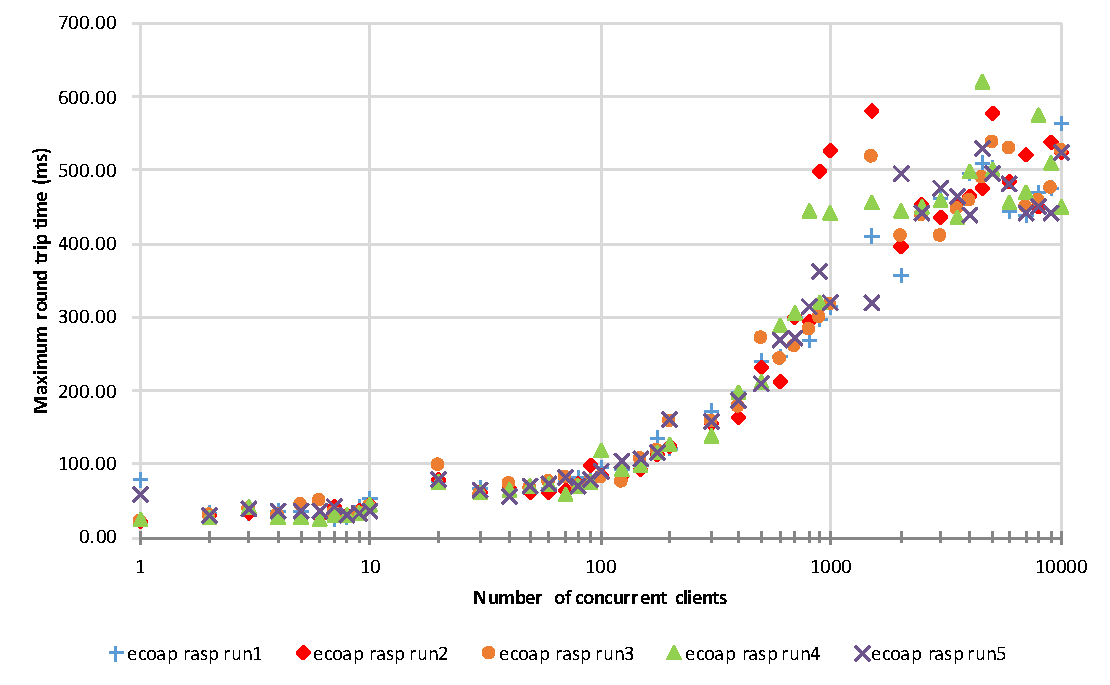
\includegraphics[scale = 0.8]{ecoap_max_round_trip_time_rasp}
\caption{Maximum round trip time of ecoap running on Raspberry Pi 3}
\label{fig:ecoap_max_round_trip_time_rasp}
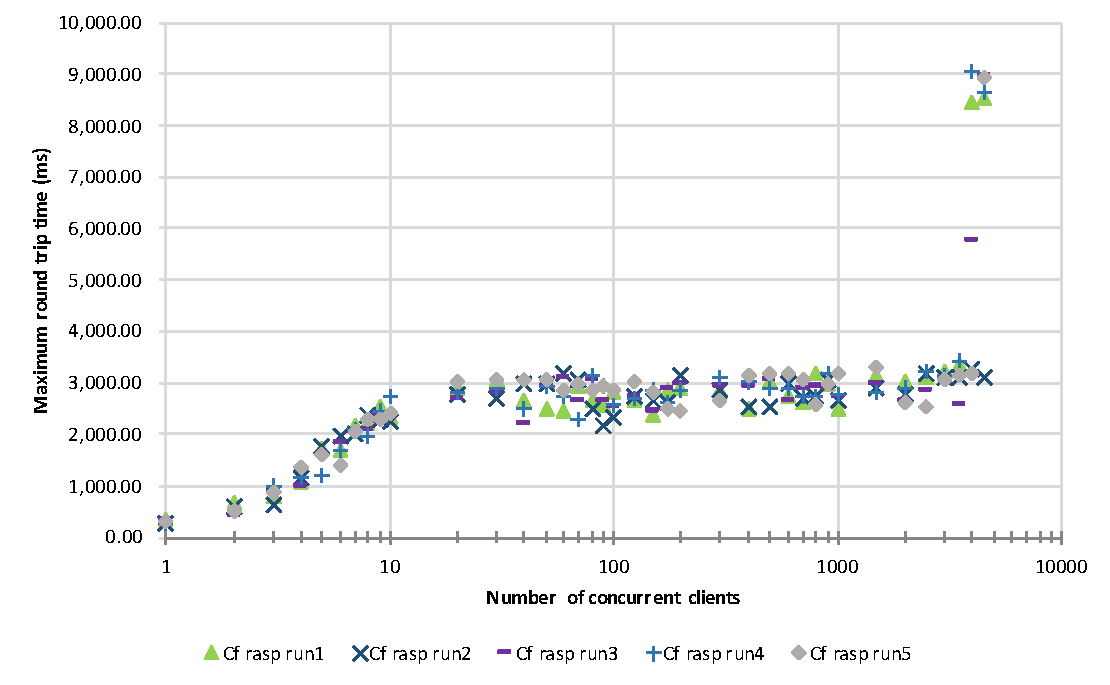
\includegraphics[scale = 0.8]{californium_max_round_trip_time_rasp}
\caption{Maximum round trip time of Californium running on Raspberry Pi 3}
\label{fig:californium_max_round_trip_time_rasp}
\end{figure}

\begin{figure}[!htbp]
\centering
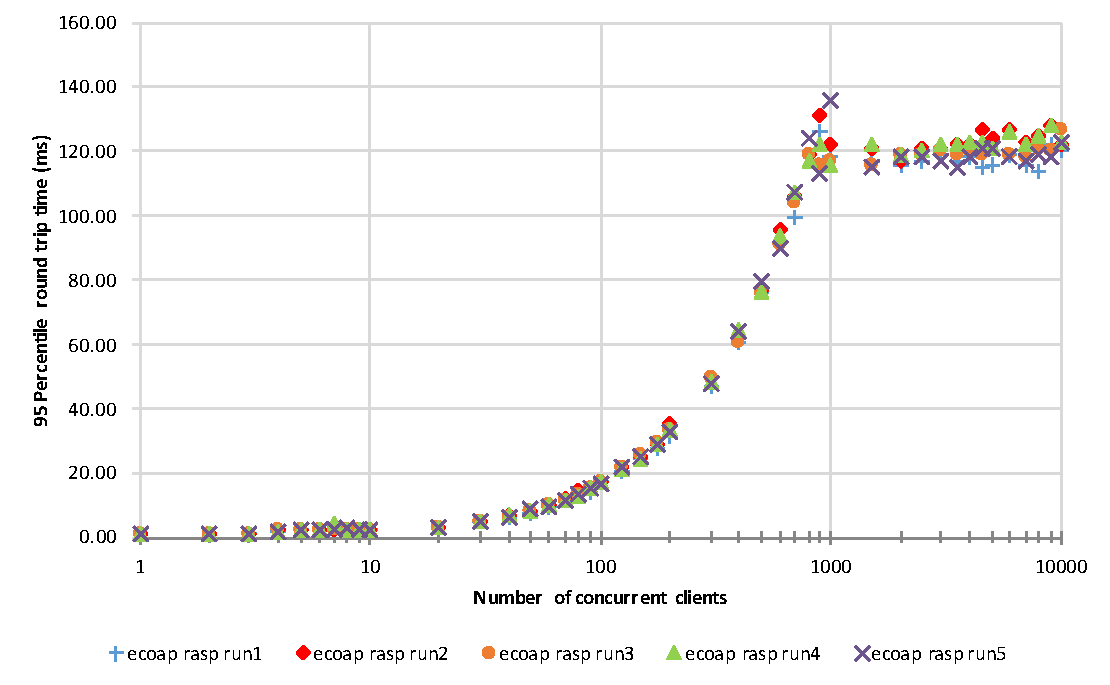
\includegraphics[scale = 0.8]{ecoap_95p_round_trip_time_rasp}
\caption{95 percentile round trip time of ecoap running on Raspberry Pi 3}
\label{fig:ecoap_95p_round_trip_time_rasp}
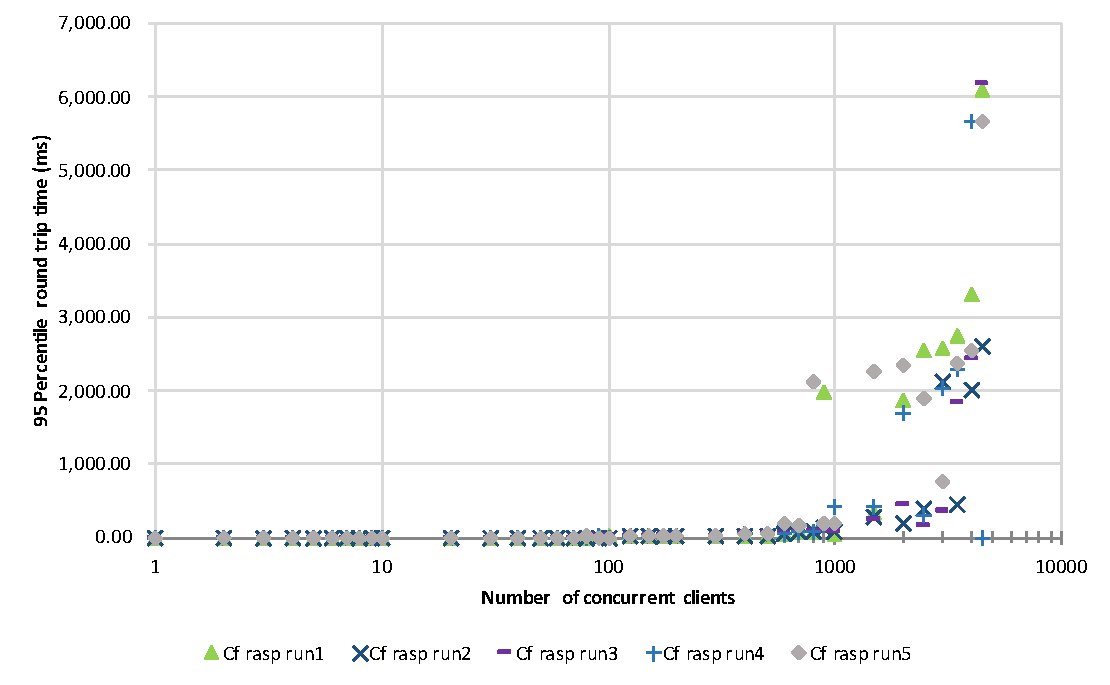
\includegraphics[scale = 0.8]{californium_95p_round_trip_time_rasp}
\caption{95 percentile round trip time of Californium running on Raspberry Pi 3}
\label{fig:californium_95p_round_trip_time_rasp}
\end{figure}

To better illustrate the soft real-time characteristics of Erlang, a separate resource \verb|\fibonacci| is hosted on the Raspberry Pi, which computes a fibonacci number in a highly inefficient recursive way using the parameter included in the request query. Then 100 virtual clients would send requests to the \verb|\fibonacci| resource in order to quickly saturate the server. Meanwhile another 100 clients would send requests to the \verb|\benchmark| resource expecting ordinary responses. The result is given in table \ref{tab:rasp_fib}. For Californium, all requests end up with timeout since the underlying threads that executes the CPU-intensive task block the whole server. However, under same load ecoap is still accessible for the non CPU-intensive requests, at the cost of increasing response time and possible more timeout messages (though not shown in this test). It is the preemptive scheduling of Erlang that ensures no process should occupy too much CPU time and improves overall responsiveness. It is of no doubt that when eventually all CPU resource has been consumed, no server could process requests normally any more. That being said, the Erlang runtime still improves the robustness of an application under heavy load compared with alternative solution, which is one desired feature for the IoT.

\begin{table}[!htbp]
\centering
\begin{tabular}{llllll}
%
 & \bfseries throughput &  \bfseries timeout & \bfseries min latency & \bfseries max latency & \bfseries 95p latency \\\hline
\bfseries Californium & 0.00 & 100\% & 0.00 & 0.00 & 0.00 \\\hline
\bfseries ecoap & 404.93 & 0\% & 13.98 & 7405.57 & 546.00\\
\end{tabular}
\caption[Result of fibonacci test on Raspberry Pi 3]{Result of fibonacci test on Raspberry Pi 3. The throughput is measured as processed requests per second. Timeout shows the percentage of lost messages in all sent messages. All latency is measured in milliseconds. Californium is not responsive so no meaningful latency is recorded while ecoap is still available at the cost of degraded performance.}
\label{tab:rasp_fib}
\end{table}

The concurrency model behind ecoap allows it to scale down to embedded platforms such as the Raspberry Pi without a problem. Since all concurrent activities are modelled as lightweight isolated processes, unnecessary synchronizations are avoided and the underlying runtime could schedule and manage the processes in a consistent manner. As a result, the benefits of fair scheduling and independent garbage collection that are discussed in unconstrained experiment also apply here and gain more explicit effects. Though other solutions can be highly customizable as well, for example, Californium supports setting different number of threads in each processing stage, as what the experiment results show, the limitations of the underlying concurrency model reduces the overall flexibility. 

\section{Fault-Tolerance Test}

Fault-tolerance is another design goal of ecoap. In order to verify the behaviour under various faults and failures, the faults need to be injected to a running server in a random manner. Chaos Monkey is a resiliency tool that helps applications tolerate random failures \cite{chaos_monkey_netflix}. It originates from Netflix and aims at testing the fault-tolerance of a a production environment by randomly terminating virtual machine instances and containers. That being said, this tool works at a coarse-grained level and does not provide finer control within one application instance. However, one Erlang application inspired by Chaos Monkey can do the trick. The application which is also called chaos monkey \cite{chaos_monkey_erl} can randomly terminate an Erlang process within another application at pre-defined rate. It therefore effectively tests the stability of the target application with any combination of failures. 

The experiment is taken with same environment as the previous AWS ones. To evaluate how fault-tolerant ecoap is, the experiment first starts the server and the benchmark tool as normal, and then randomly kills a process of the server for every 2 seconds during an ongoing stress test. The interval of 2 seconds is the minimum value that can be used respecting the restart limit of supervisors inside ecoap. The chaos monkey is smart enough to only kill worker processes because it is where the majority of errors happen, while the supervisors are too strong to kill. Usually the crash of a supervisor implies an unrecoverable error just occurred and the entire supervision tree is abandoned. 

In such a way, the throughput of the server under ``attack" is shown in figure \ref{fig:throughput_with_faults}. It can be seen clearly that when the chaos monkey application is active, the standard deviation gets quite large at low concurrency level. This is because with low concurrency factor, fewer processes run in the server and kill one of them every 2 seconds is considered a non-negligible obstacle. The server survives the attack but can not run as stable as usual. Nevertheless, the situation gets better when more concurrent clients are involved, since a system with larger amount of processes is naturally resilient to fixed rate failure. Therefore, the throughput becomes closer to the one without any fault as the number of concurrent clients grows. 

Figure \ref{fig:ecoap_min_round_trip_time_faults}, \ref{fig:ecoap_max_round_trip_time_faults} and \ref{fig:ecoap_95p_round_trip_time_faults} show the minimum, maximum and 95 percentile latency during the test respectively. It should be noticed that compared with the data with no fault, only slight difference exists. The server is overall not greatly influenced by the injected faults. On the other hand, message timeout rate does not provide much information here. Though with injected faults there are message timeouts from the beginning of the test, the timeout percentage is in general similar to normal one or even lower. This is reasonable because the virtual clients work in a closed-loop fashion. The clients send fewer requests in total as a result of the faults, so as the number of timeout messages. Thus the percentage of lost messages will not change dramatically.

It is interesting enough to see that ecoap can keep providing service with such a high failure rate. Moreover, since the killed process is randomly selected, the experiment should prove that the system is strongly recoverable and resilient no matter which stage went wrong. Without Erlang's share-nothing isolation and supervision tree mechanism, this fine-grained fault-tolerance is hard to achieve. It can be perceived that the high reliability of single node would make it easier to build a high availability multi-node system.

Similar tests can not be conducted with Californium, as it makes no sense to randomly terminate a thread within a threading concurrency model. This also means that in order to improve reliability, application with traditional model must use defensive programming, carefully managed locks and asynchronous calls. It may fits specific circumstances very well and outperform the proposed concurrency model, however, it is essentially not as intuitive as the latter and one has to pay the maintainability overhead and loss of flexibility eventually.

\begin{figure}[!htbp]
\centering
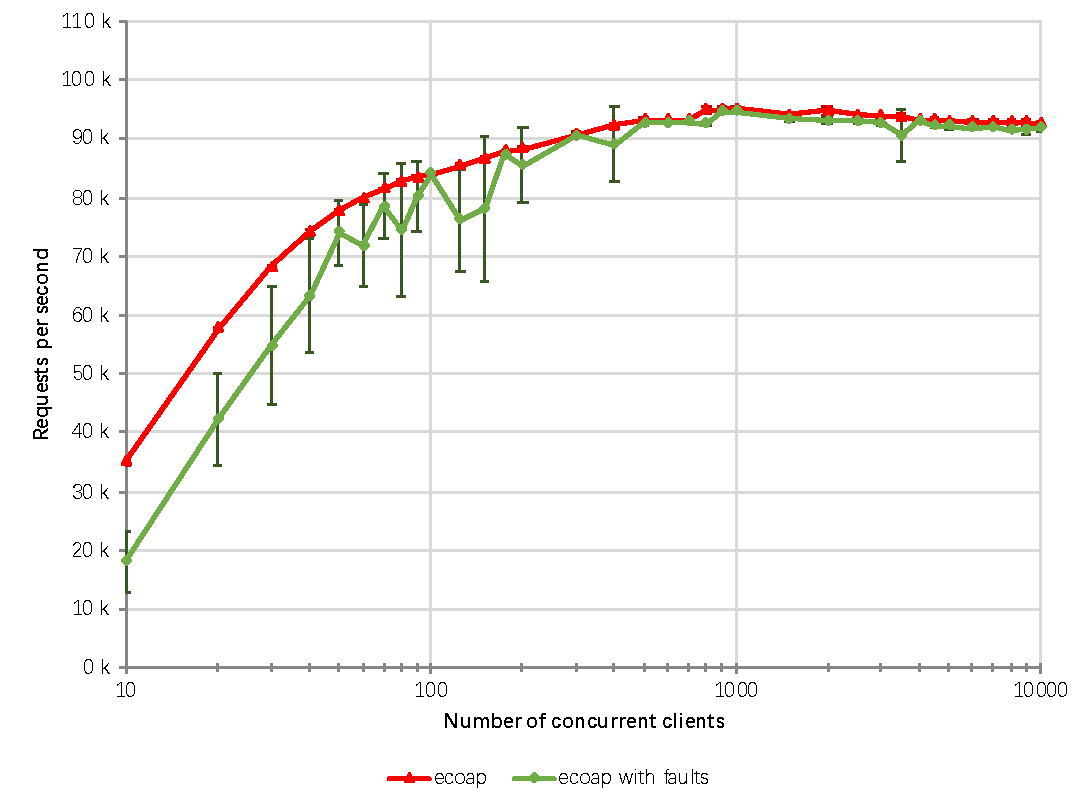
\includegraphics[scale = 0.8]{throughput_with_faults}
\caption[Throughout of ecoap with randomly injected faults]{Throughout of ecoap with randomly injected faults. The chaos monkey application randomly kill a worker process of ecoap every 2 seconds. The performance is more disturbed at low concurrency factor.}
\label{fig:throughput_with_faults}
\end{figure}

\begin{figure}[!htbp]
\centering
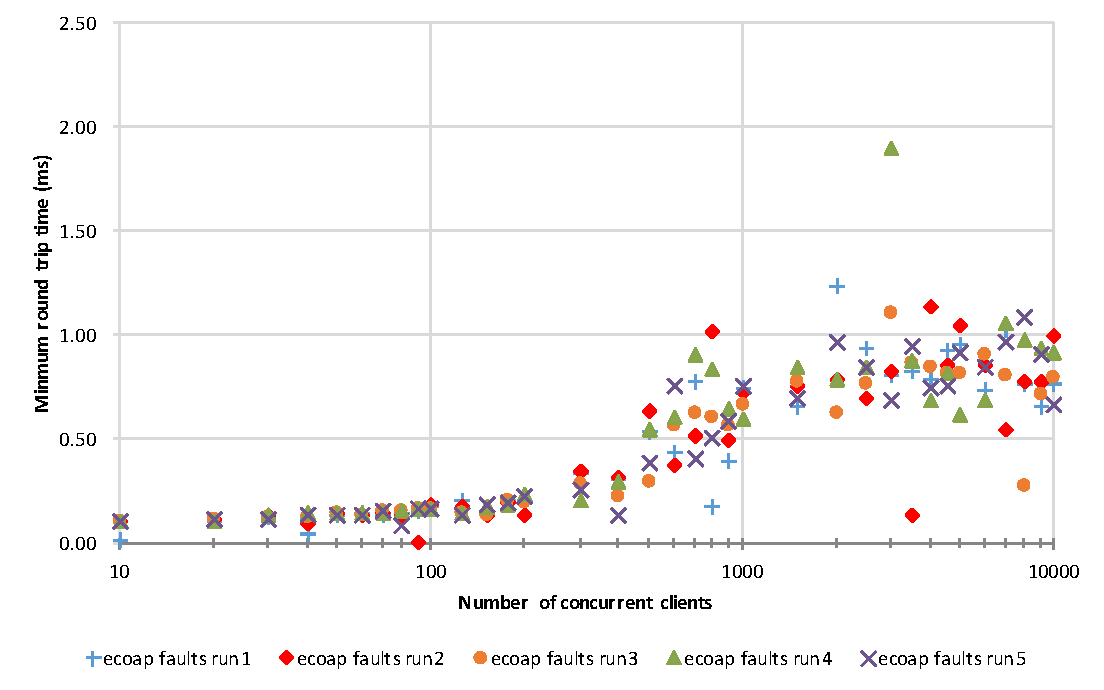
\includegraphics[scale = 0.8]{ecoap_min_round_trip_time_faults}
\caption{Minimum round trip time of ecoap with randomly injected faults}
\label{fig:ecoap_min_round_trip_time_faults}
\end{figure}

\begin{figure}[!htbp]
\centering
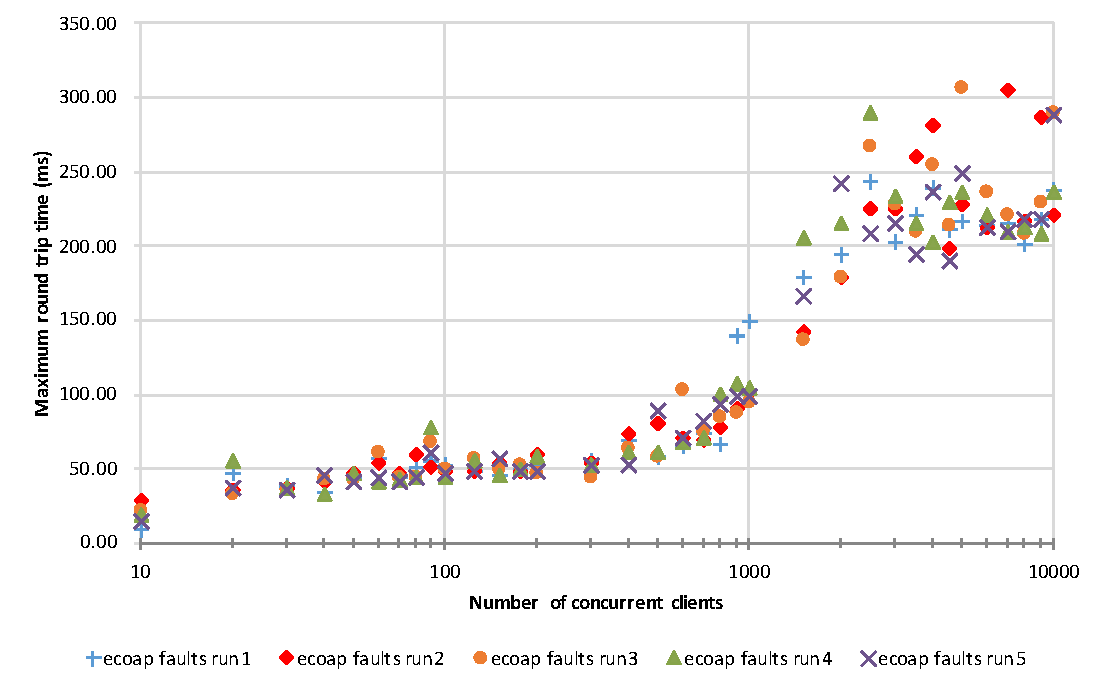
\includegraphics[scale = 0.8]{ecoap_max_round_trip_time_faults}
\caption{Maximum round trip time of ecoap with randomly injected faults}
\label{fig:ecoap_max_round_trip_time_faults}
\end{figure}

\begin{figure}[!htbp]
\centering
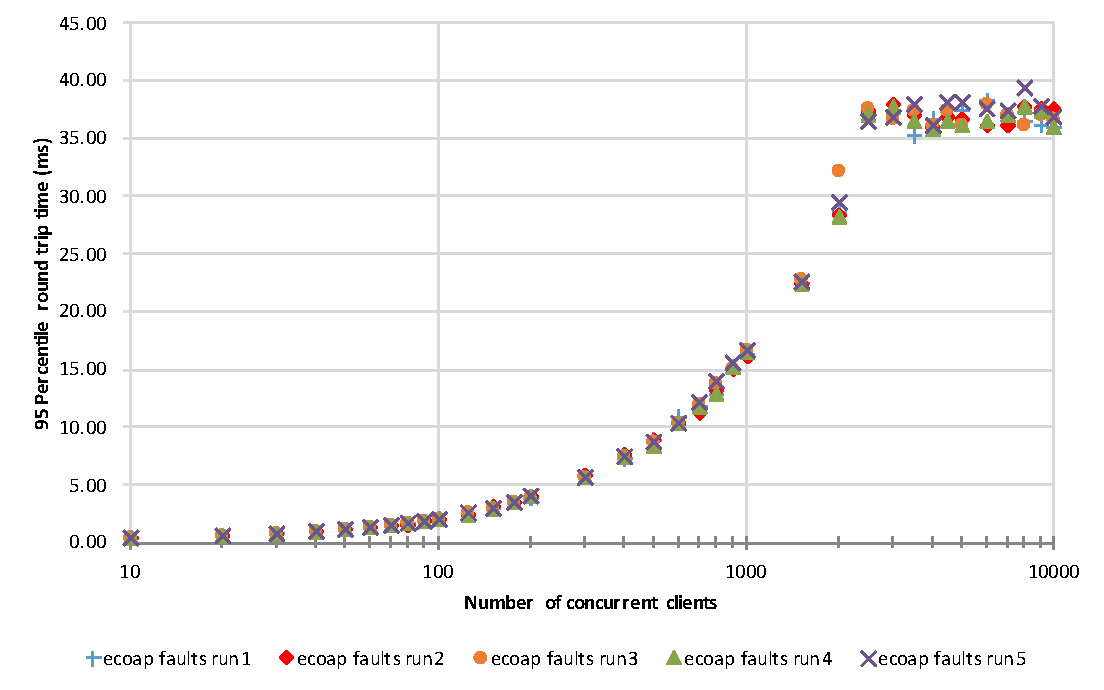
\includegraphics[scale = 0.8]{ecoap_95p_round_trip_time_faults}
\caption{95 percentile round trip time of ecoap with randomly injected faults}
\label{fig:ecoap_95p_round_trip_time_faults}
\end{figure}

\section{Summary and Discussion}

This chapter answers the question how CoAP can be efficiently implemented using a concurrency-oriented language like Erlang, and how the system can automatically scale up to powerful cloud environment as well as scale down to constrained platform. The ecoap prototype gives an architecture for scalable and reliable IoT services. Furthermore, a detailed evaluation of the proposed prototype in both constrained and unconstrained environment is presented. The ecoap prototype consists of reusable components for both server and client, which then forms a flexible concurrency model where protocol processing is clearly divided and parallelized. Details of different components and how they work together are also explained in this chapter, with an emphasis on modelling and managing various states efficiently within CoAP constraints. The evaluation shows that the concurrency model fits modern multi-core systems well. The implementation has similar or better performance compared with mainstream CoAP solution. 

In unconstrained environment, ecoap has similar level of scalability as Californium with respect to a growing number of concurrent clients. Both implementations maintain a high throughout even with high concurrency factor and only latency increases. However, ecoap gives in general more stable and responsive performance as a result of the underlying concurrency model. The latency results indicate that ecoap is more suitable for applications with real-time requirements, since it ensures the worst cases are still within an acceptable range. 

In constrained environment, ecoap outperforms Californium in both throughput and latency. It automatically scales down without extensive optimization while keeping consistent behaviour as in unconstrained environment. Solutions like Californium may have a concurrency model that is more advanced in certain scenarios, however, they might not benefit from it when the environment changes. ecoap and its concurrency model gain more flexibility in general.

Moreover, ecoap is more resilient in terms of unexpected faults and failures. The fine-grained control over errors and faults and recover process can not be easily achieved in other solutions. 
As the number of participants of the IoT increases rapidly, such feature becomes more important because it gives more alternatives to achieve reliability. 



%what can the readers learn from your work -> the real conclusion!
